% ============================================================
% Apex Trays — Integrated Cartridge-Grid Distillation Stage
% HyTray Invention Disclosure Series
% ============================================================
\documentclass[11pt,letterpaper]{article}

% ── packages ─────────────────────────────────────────────────────────────────
\usepackage[top=1.0in, bottom=1.0in, left=1.0in, right=1.0in]{geometry}
\usepackage{amsmath,amssymb}
\usepackage{booktabs}
\usepackage{graphicx}
\usepackage[colorlinks=true,linkcolor=blue!60!black,citecolor=blue!60!black,
            urlcolor=blue!60!black]{hyperref}
\usepackage[separate-uncertainty=true]{siunitx}
\DeclareSIUnit\inch{in.}
\DeclareSIUnit\psi{psi}
\DeclareSIUnit\ft{ft}
\usepackage{tabularx}
\usepackage{longtable}
\usepackage{caption}
\usepackage{subcaption}
\usepackage{fancyhdr}
\usepackage{enumitem}
\usepackage{array}
\usepackage{multirow}
\usepackage{float}
\usepackage{microtype}
\usepackage{parskip}
\usepackage{xcolor}

% ── page style ───────────────────────────────────────────────────────────────
\pagestyle{fancy}
\fancyhf{}
\rhead{\small HyTray Invention Disclosure Series}
\lhead{\small Apex Trays}
\cfoot{\small\thepage}
\renewcommand{\headrulewidth}{0.4pt}

% ── math short-hands ─────────────────────────────────────────────────────────
\newcommand{\Csb}{C_{\mathrm{SBF}}}
\newcommand{\FLV}{\mathrm{FLV}}
\newcommand{\dpd}{\Delta P_{\mathrm{dry}}}
\newcommand{\dpt}{\Delta P_{\mathrm{tray}}}
\newcommand{\dptot}{\Delta P_{\mathrm{total}}}
\newcommand{\how}{h_{\mathrm{ow}}}
\newcommand{\hcl}{h_{\mathrm{cl}}}
\newcommand{\hdc}{h_{\mathrm{dc}}}
\newcommand{\eoc}{E_{\mathrm{OC}}}
\newcommand{\etray}{E_{\mathrm{tray}}}
\newcommand{\unf}{u_{\mathrm{nf}}}
\newcommand{\udesign}{u_{\mathrm{design}}}

% ── caption formatting ────────────────────────────────────────────────────────
\captionsetup{font=small,labelfont=bf}

% ════════════════════════════════════════════════════════════════════════════
\begin{document}

% ── title block (mimicking HT-0X datasheet layout) ──────────────────────────
\begin{center}
  {\large\bfseries HyTray Invention Disclosure Series}\\[4pt]
  {\LARGE\bfseries Apex Trays: An Integrated Cartridge-Grid\\
  Distillation Stage}\\[8pt]
  {\large A deck combining five HT-series mechanisms to improve\\
  capacity, turndown, efficiency and fouling resistance\\
  relative to conventional cross-flow tray families}\\[10pt]
  \textit{Inventor:} Pratik\\[4pt]
  \textit{Invention Disclosure / Provisional Specification Draft --- HyTray Series HT-AP}\\
  June 2026
\end{center}

\hrule\vspace{6pt}

% ── abstract ─────────────────────────────────────────────────────────────────
\begin{abstract}
\noindent
A distillation-column tray is disclosed that integrates five separately
patentable HyTray mechanisms --- HT-02/HT-08 swirl-tube cartridges
(primary contacting zone, $\approx$70\% of active area), HT-01C lip-sealed
trickle valves (secondary zone, $\approx$15\%), HT-03 GRADEX
radial/azimuthal vapour-load grading, HT-05 PULSAR self-sweeping
oscillator relief slots, and HT-07 AEGIS bolted structural
cartridge-grid --- into a single bolt-in deck designated
\textbf{Apex Trays}.  The five mechanisms address conflicting design goals
(capacity, turndown, fouling resistance, structural rating, efficiency)
by assigning each goal a dedicated zone or deck-level treatment, rather
than attempting a single-geometry compromise.  A first-order hydraulics
model (Fair flooding correlation, orifice-equation dry-tray pressure drop,
Francis-weir liquid height, downcomer backup, O'Connell efficiency)
predicts the following results at the General Rectification design point,
relative to a plain sieve tray sized on the same basis: column diameter
reduced by 39\%, total column pressure drop reduced by 54\%, operating-range
turndown increased from 2.0:1 to 22.2:1, tray efficiency increased from
76.2\% to 91.4\%, dry-tray pressure drop increase under fouling reduced
from $+$78\% to $+$16\%, and first-order relative installed cost reduced
by 36\%.  Consistent 39\% diameter reductions are obtained across five
representative services (general rectification, fouling/heavy-ends,
vacuum, high-pressure/high-liquid-load, foaming).  All results are
model predictions based on independently published correlations and
parametric TrayType factors; they require experimental and CFD validation.
\end{abstract}

\noindent\textit{Status:} All performance figures are predictions from a
one-dimensional hydraulics model (\texttt{column\_hydraulics.py}) using
parameterised TrayType factors (\texttt{tray\_library.py}).  The model
applies the same Fair/Kister correlation framework to every tray family;
the differences between trays arise entirely from their TrayType parameter
sets (Table~\ref{tab:traytype}).  Physical mechanisms such as centrifugal
disengagement (swirl tubes) and lip-seal trickle behaviour (HT-01C) are not
resolved by a 1-D model; the claimed capacity factor ($k_{\mathrm{cap}}=2.50$)
and minimum stable load fraction ($f_{\mathrm{min}}=0.045$) are design targets
that require validation in a cold-flow or hot pilot rig.

\hrule\vspace{6pt}

% ── table of contents ────────────────────────────────────────────────────────
\tableofcontents
\newpage

% ════════════════════════════════════════════════════════════════════════════
\section{Field of the Invention}

Vapour--liquid contacting internals for distillation and absorption columns,
specifically a cross-flow tray designed to increase column throughput,
extend stable operating range, reduce pressure drop, improve tray efficiency
and resist fouling fouling, while remaining removable through a standard
manway and installable without column modifications beyond nozzle re-rating.

% ════════════════════════════════════════════════════════════════════════════
\section{Background and Prior Art}

Conventional cross-flow trays (sieve, valve, fixed-valve, dual-flow) face a
set of competing design constraints that have not been resolved simultaneously
by any single mechanism:

\begin{itemize}[nosep]
  \item \textbf{Capacity} is bounded by the Souders-Brown entrainment-flooding
    criterion, $u < \Csb\sqrt{(\rho_L-\rho_V)/\rho_V}$, where
    $\Csb\approx\SI{0.08}{\metre\per\second}$ for conventional cross-flow
    geometry at 24-inch spacing.  High-capacity decks
    (Koch-Glitsch SUPERFRAC\textsuperscript{\textregistered},
    Sulzer VGPlus) recover some active area from the downcomers but remain
    gravity-limited.

  \item \textbf{Fouling resistance} favours large, simple openings (Kister:
    round holes $>\SI{12}{\milli\metre}$ resist plugging best) and no
    moving parts.  High-capacity designs favour small, precisely shaped
    elements --- in tension with fouling resistance.

  \item \textbf{Turndown} requires a secondary low-load flow path that
    stays open when the primary perforations weep.  Dual-flow trays
    achieve good open area but lose downcomer action and have limited
    turndown of roughly 1.5:1.  Moving valve trays reach approximately
    3.3:1 but at higher hardware cost.

  \item \textbf{Structural rating} against vapour uplift transients (1--5 psi)
    requires thick plate and dense beam grids that cost open area.

  \item \textbf{Tray efficiency} is improved by cross-flow uniformity, liquid
    path length, and froth height, but increased froth height raises pressure
    drop.
\end{itemize}

Prior high-capacity decks (SUPERFRAC, UFM, VGPlus) address capacity and
partial fouling resistance but do not simultaneously extend turndown beyond
roughly 2.5:1 or provide a structural uplift rating integrated with the
active deck.  Swirl-tube contactors (Shell ConSep class) decouple flooding
from tray spacing but typically feed liquid from dedicated downcomer hardware
and do not integrate a secondary low-load trickle path.

% ════════════════════════════════════════════════════════════════════════════
\section{Objects of the Invention}

\begin{enumerate}[nosep]
  \item To provide a tray whose vapour-capacity flood point is controlled by
    centrifugal mechanical disengagement rather than gravity settling, targeting
    a capacity factor $k_{\mathrm{cap}}\geq 2.0$ relative to the Fair sieve
    baseline at equal tray spacing.
  \item To achieve a stable operating range from minimum load (weep point) to
    flood that spans at least 15:1 turndown, by pairing a primary swirl-tube
    zone with a secondary lip-sealed trickle zone that engages at low vapour
    rate.
  \item To reduce wet-tray pressure drop relative to a sieve tray of equivalent
    theoretical-stage-count through a combination of low-height weirs
    ($h_{\mathrm{weir}}=\SI{0.5}{\inch}$), high open-area fraction
    ($f_{\mathrm{hole}}=0.25$) and mechanically lean froth (aeration factor
    $\beta=0.38$).
  \item To achieve high open-area retention under fouling conditions
    ($f_{\mathrm{foul}}\geq 0.90$) by using wide, unobstructed slot openings
    swept by a self-oscillating relief mechanism (HT-05 PULSAR).
  \item To improve tray efficiency above the O'Connell baseline through
    radial/azimuthal vapour-load grading (HT-03 GRADEX) and multi-chordal
    liquid sweeping, targeting an efficiency factor of $\eta=1.20$.
  \item To provide structural uplift resistance of 2--5\,psi without
    reducing active-area fraction below 85\%, by mounting the deck on a
    bolted cartridge-grid (HT-07 AEGIS) with integral hook clamps and relief
    flaps.
  \item To allow deck renewal in a column turnaround by bolt-in/bolt-out
    cartridge exchange through the column manway, without shell modification.
\end{enumerate}

% ════════════════════════════════════════════════════════════════════════════
\section{Summary of the Invention}

Apex Trays comprise a single deck panel supported by a bolted structural
cartridge-grid (AEGIS, item~6 in the objects above).  The active area
($f_{\mathrm{active}}=0.85$ of the column cross-section) is divided into two
contacting zones:

\begin{description}[nosep]
  \item[Primary zone (\texttildelow 70\% of $A_{\mathrm{col}}$)]
    An array of short swirl-tube cartridges (HT-02/HT-08 VORTEXA) on a
    triangular pitch.  Each cartridge comprises a vertical tube
    (80--150\,mm~ID) with 4--8 tangential vapour slots, liquid-metering ports
    from the deck pool, and a fixed vane cap for centrifugal
    vapour--liquid disengagement at 30--60\,$g$.
    HT-08 VORTEXA's back-drivable helical sleeve passively modulates slot
    area with vapour rate, extending the primary zone's own stable range.

  \item[Secondary zone (\texttildelow 15\% of $A_{\mathrm{col}}$)]
    Lip-sealed dual-flow valves (HT-01C LipSeal) that provide a dedicated
    low-vapour-rate trickle path.  The LipSeal lips seat against weep at
    loads below roughly $f_{\mathrm{min,sec}}\approx 0.04$ of the design
    throughput.  When the primary zone is throttled at low load, the secondary
    zone sustains vapour--liquid contact and prevents column weeping.
\end{description}

Three deck-wide treatments are superimposed on both zones:

\begin{description}[nosep]
  \item[GRADEX (HT-03)] Radial and azimuthal cartridge-pitch grading and
    multi-chordal liquid baffling to equalize the vapour--liquid ratio across
    the tray, eliminating concentration gradients and dead zones.
  \item[PULSAR (HT-05)] Self-sweeping oscillator relief slots between
    cartridges that briefly open under a pressure differential, dislodging
    deposits from the slot edges and reducing fouling accumulation.
  \item[AEGIS (HT-07)] Bolted structural cartridge-grid below the deck,
    carrying the deck in tension via hook clamps to resist vapour uplift of
    2--5\,psi.  Integral relief flaps in the grid crack at a set differential
    to bound the sustained structural load.
\end{description}

% ════════════════════════════════════════════════════════════════════════════
\section{Brief Description of Figures}

\begin{description}[nosep]
  \item[Figure~\ref{fig:cross_section}] Apex deck cutaway elevation at the
    General Rectification design point ($D=\SI{32}{\inch}$, 24-inch tray
    spacing).  Shows the primary swirl-tube zone, secondary lip-seal trickle
    zone, PULSAR relief slots, AEGIS structural grid, and downcomer.
  \item[Figure~\ref{fig:plan_view}] Plan view (top-down) of Apex deck,
    showing hex-packed cartridges in the primary zone with GRADEX radial
    shading and the secondary lip-seal zone adjacent to the downcomers.
  \item[Figure~\ref{fig:family_cross_sections}] Seven-panel schematic
    cross-section comparison of all tray families: Sieve, Dual-Flow, Moving
    Valve, Fixed Valve, High-Performance Multi-Downcomer, Ripple (Corrugated),
    and Apex.
  \item[Figures~\ref{fig:diameter}--\ref{fig:cost}] Service-comparison charts:
    column diameter, total pressure drop, turndown and efficiency, relative
    installed cost, and fouling sensitivity --- all seven trays across five
    representative services.
\end{description}

% ════════════════════════════════════════════════════════════════════════════
\section{Detailed Description}
\label{sec:detailed}

\subsection{Architecture Overview}
\label{sec:architecture}

Apex's active area ($f_{\mathrm{active}}=0.85$) is partitioned as follows
(numbers refer to the General Rectification design point, $D=\SI{32}{\inch}$):

\begin{center}
\small
\begin{tabular}{lccccc}
\toprule
Zone / treatment & Fraction of $A_{\mathrm{col}}$ & $A$ (ft$^2$)
  & $A$ (in$^2$) & Open area (ft$^2$) & Open area (in$^2$)\\
\midrule
Primary (HT-02/HT-08 cartridges) & 0.70 & 3.88 & 559 & 0.97 & 140\\
Secondary (HT-01C lip-seal)       & 0.15 & 0.83 & 120 & 0.21 &  30\\
Downcomers (both sides)           & 0.15 & 0.83 & 120 & ---  & ---\\
\textbf{Active total}             & \textbf{0.85} & \textbf{4.72} & \textbf{679}
  & \textbf{1.18} & \textbf{170}\\
\bottomrule
\end{tabular}
\end{center}

At the design point: hole velocity $u_{\mathrm{hole}}=\SI{12.14}{ft/s}$;
dry-tray $\dpd=1.29$\,in.\,liq; clear-liquid height
$\hcl=1.42$\,in. (weir 0.50\,in. plus Francis crest 0.92\,in.);
total wet-tray $\dpt=0.0317$\,psi.

\subsection{Primary Contacting Zone: Swirl-Tube Cartridges (HT-02/HT-08 VORTEXA)}
\label{sec:primary}

Each cartridge is a vertical tube of 80--150\,mm ID and height 1.2--2.0
diameters, mounted in the deck on a triangular pitch of 1.4--1.7 tube
diameters.  Vapour enters through 4--8 tangential slots at 18--35\,m/s,
generating a Rankine-type vortex at swirl number $S=1.5$--3.0 and wall
centripetal acceleration 30--60\,$g$.  Liquid is fed from the surrounding
deck pool through 3--6 calibrated metering ports (8--14\,mm diameter), which
behave as submerged orifices:
\begin{equation}
  Q_p = C_d A_p \sqrt{2g h_{\mathrm{cl}}}, \quad C_d \approx 0.62,
  \label{eq:port_flow}
\end{equation}
maintaining per-tube liquid rates of 1.5--4.0\,m$^3$/h and a film Reynolds
number $Re_f = 4\Gamma/\mu_L$ of 1500--8000.  A vane crown separator at the
tube exit (8--16 vanes at 35--55\ensuremath{^\circ}) slings separated liquid
into a collection annulus draining directly to the outlet-weir region,
bypassing the active deck and preventing re-entrainment.

HT-08 VORTEXA adds a back-drivable helical sleeve that passively opens slot
area with increasing vapour load (axial lift proportional to momentum flux)
and closes it at low load, extending the primary zone's stable range from
$\approx$2.5:1 (fixed-geometry HT-02) to $\approx$8:1 before the zone
approaches weep.  A seized sleeve reverts to fixed-geometry HT-02 behaviour,
with no cascading failure mode.

\subsection{Secondary Contacting Zone: LipSeal Trickle Path (HT-01C)}
\label{sec:secondary}

The secondary zone ($\approx$15\% of $A_{\mathrm{col}}$) comprises HT-01C
dual-flow lip valves.  Each valve is a circular flap seated by spring or
gravity; the lip face seals against the deck orifice edge when net upward
vapour force is below the seating load, preventing liquid weeping.  At
moderate-to-high throughput both zones contact normally.  At low vapour rate,
when the primary swirl tubes under-perform, the secondary zone sustains
vapour--liquid contact; the LipSeal lip prevents liquid dump-through and
maintains a contact froth even at column throughputs as low as 4--5\% of
the primary-zone design basis.  This two-zone hand-off is the primary
mechanism behind Apex's \texttt{min\_load\_frac} = 0.045 and the resulting
22.2:1 turndown --- a parameter that is the single largest modelling
uncertainty and cannot be verified by the 1-D engine used here.

\subsection{Radial and Azimuthal Grading (HT-03 GRADEX)}
\label{sec:gradex}

GRADEX superimposes a variable cartridge pitch and/or variable slot count on
the primary zone, targeting a uniform vapour/liquid ratio across the tray
radius.  In a standard sieve tray, the liquid flow path from the inlet to the
outlet weir creates a positive vapour-flow gradient (more vapour near the
outlet due to lower liquid head) that reduces local efficiency by 5--10
percentage points relative to the stage-wise ideal.  GRADEX counters this by
setting closer cartridge pitches (higher vapour-path area per unit plan area)
near the liquid inlet and looser pitches near the outlet weir.  Multi-chordal
liquid baffles sweep the tray in three or four chords rather than a single
long path, reducing the concentration gradient along each chord and preventing
stagnant corner zones.  The combined effect is captured in the model by
\texttt{efficiency\_factor} = 1.20 --- a 20\% uplift on the O'Connell
baseline, compared to 0\% for sieve, moving-valve and fixed-valve trays and
10\% for Ripple (corrugated) trays.

\subsection{Self-Sweeping Oscillator Relief Slots (HT-05 PULSAR)}
\label{sec:pulsar}

PULSAR slots are elongated relief openings located in the deck plate between
cartridge footprints.  Each slot is held closed by a spring-loaded or
weight-loaded cap that briefly opens when the deck differential pressure
exceeds a set value (typically 10--30\,mbar above normal tray $\Delta P$).
The brief high-velocity vapour jet through the slot mechanically dislodges
deposits from the slot edge and surrounding deck surface, then the cap
reseats.  Because the opening is pressure-actuated and self-reseating, it
contributes no parasitic pressure drop or vapour bypass during normal
operation.  PULSAR is modelled through \texttt{fouling\_open\_area\_retention}
= 0.93 --- the fractional open area retained after fouling --- compared to
0.75 for sieve and 0.70 for moving valve.  The 93\% retention predicts a dry-tray
pressure drop increase of $+$16\% under fouling versus $+$78\% for sieve.

\subsection{Structural Cartridge-Grid (HT-07 AEGIS)}
\label{sec:aegis}

The AEGIS grid is a welded below-deck structural frame to which each cartridge
and deck panel is attached by hook clamps engaging a support ring.  The
geometry follows HT-07's parametric design (see separate HT-07 disclosure):
deck panels of 2.0--3.0\,mm stainless steel with stiffening ribs at pitch
$s \leq t\sqrt{\sigma_{\mathrm{allow}}/(0.75\,q)}$, where $t$ is deck
thickness, $\sigma_{\mathrm{allow}}$ is the plate allowable stress, and
$q$ is the design uplift pressure (21--34.5\,kPa, i.e.\ 3--5\,psi).  For
$t=2.5$\,mm, $\sigma_{\mathrm{allow}}=140$\,MPa and $q=34.5$\,kPa, the
maximum rib pitch is 184\,mm; a 170\,mm pitch is adopted.  The rib footprint
consumes $<4$\% of bubbling area.  Integral relief flaps (5--10\% of tray
area) crack at 1.5--2\,psi to cap the sustained structural load.  Because the
cartridges are bolted to the grid and the grid is bolted to the support ring,
the entire active deck can be exchanged in a turnaround without cutting or
re-welding the column shell.

\subsection{Hydraulic Design Equations}
\label{sec:hydraulics}

The following equations are implemented in \texttt{column\_hydraulics.py} and
are applied identically to every tray family in the comparison.
The only quantities that differ between trays are the TrayType parameters
(Table~\ref{tab:traytype}).  All units are US customary (FPS) unless noted;
conversion factors are stated inline.

\subsubsection{Flow Parameter}
\label{sec:flv}

The dimensionless Souders-Brown flow parameter:
\begin{equation}
  \FLV = \frac{L}{V}\sqrt{\frac{\rho_V}{\rho_L}}
  \label{eq:flv}
\end{equation}
where $L$, $V$ are liquid and vapour mass flows (lb/hr) and $\rho_L$,
$\rho_V$ are the corresponding phase densities (lb/ft$^3$).  $\FLV$ is the
abscissa of Fair's flooding-correlation chart; it ranges from $\approx$0.01
for dilute-vapour vacuum services to $\approx$1.0 for high-pressure
liquid-loaded services (e.g.\ the C$_3$/C$_4$ splitter case).

\subsubsection{Fair Capacity Parameter}
\label{sec:csbf}

The closed-form fit to Fair's (1961) $\Csb$ chart, as widely used in
process simulators and following Kister \textit{Distillation Design} (1992):
\begin{equation}
  \Csb\,[\mathrm{m/s}] = 0.0105 + 8.127\times10^{-4}\,
  H_S[\mathrm{mm}]^{0.755}\,
  \exp\!\bigl(-1.463\,\FLV^{0.842}\bigr)
  \label{eq:csbf}
\end{equation}
where $H_S$ is the tray spacing in millimetres.  Valid range:
$H_S = 150$--600\,mm (6--24\,inch), $\FLV = 0.01$--1.0.  $\Csb$ is converted
to ft/s by multiplying by 3.28084.  This is identical for all trays at a
given service; tray-specific capacity differences enter in the next step.

\subsubsection{Flooding Velocity}
\label{sec:unf}

Souders-Brown flooding velocity, corrected for surface tension and modified
by the tray's capacity factor $k_{\mathrm{cap}}$:
\begin{equation}
  \unf = \Csb\left(\frac{\sigma}{\sigma_{\mathrm{ref}}}\right)^{0.2}
         \sqrt{\frac{\rho_L-\rho_V}{\rho_V}}
         \times k_{\mathrm{cap}} \times k_{\mathrm{sys}}
  \label{eq:unf}
\end{equation}
where $\sigma$ is the liquid surface tension (dyn/cm), $\sigma_{\mathrm{ref}}
= 20$\,dyn/cm (the reference value for Fair's original chart), $k_{\mathrm{cap}}$
is the tray's capacity factor (1.00 for sieve, 2.50 for Apex), and $k_{\mathrm{sys}}$
is the system (foaming) derate applied uniformly to all trays (1.00 for
non-foaming services, 0.75 for the foaming case).

\paragraph{Physical basis of $k_{\mathrm{cap}} = 2.50$ for Apex.}
In a plain sieve tray, the $\Csb$ limit is set by the droplet settling
criterion: a droplet of velocity $v_t$ settles if the vapour superficial
velocity $u < v_t \propto \Csb\sqrt{(\rho_L-\rho_V)/\rho_V}$.  The swirl-tube
cartridges subject the vapour--liquid dispersion to centripetal acceleration
$a = 30$--60\,$g$; the effective settling velocity in the tube scales as
$v_{t,\mathrm{centrifugal}} \sim v_t\sqrt{a/g}$, giving a capacity gain
of $\sqrt{30\text{--}60} = 5.5$--7.7 relative to gravity settling.  The
value $k_{\mathrm{cap}}=2.50$ is the net deck-level gain after accounting for
the 70\% area fraction of the primary zone and the secondary zone's lower
capacity; it is an engineering estimate pending hot-rig validation.

\subsubsection{Design Velocity, Area and Column Diameter}
\label{sec:sizing}

\begin{align}
  \udesign &= f_{\mathrm{flood}}\,\unf
  \label{eq:udesign}\\
  A_{\mathrm{active}} &= \frac{\dot{V}}{\udesign}, \quad
  \dot{V}\,[\mathrm{ft}^3/\mathrm{s}] = \frac{V\,[\mathrm{lb/hr}]}
    {3600\,\rho_V\,[\mathrm{lb/ft}^3]}
  \label{eq:aactive}\\
  A_{\mathrm{col}} &= \frac{A_{\mathrm{active}}}{f_{\mathrm{active}}}
  \label{eq:acol}\\
  D &= \sqrt{\frac{4\,A_{\mathrm{col}}}{\pi}}
  \label{eq:diameter}
\end{align}

$f_{\mathrm{flood}} = 0.80$ throughout, except the Fouling service
($f_{\mathrm{flood}} = 0.65$).  The diameter reduction of Apex relative to
sieve at equal $f_{\mathrm{flood}}$ follows directly from
Equations~\eqref{eq:unf}--\eqref{eq:diameter}:
\begin{equation}
  \frac{D_{\mathrm{Apex}}}{D_{\mathrm{Sieve}}} =
  \frac{1}{\sqrt{k_{\mathrm{cap}}\times f_{\mathrm{active,Apex}}/f_{\mathrm{active,Sieve}}}}
  = \frac{1}{\sqrt{2.50\times 0.85/0.78}} = \frac{1}{\sqrt{2.724}} = 0.606
  \label{eq:dratio}
\end{equation}
i.e.\ a 39.4\% diameter reduction, consistent with Table~\ref{tab:apex_sieve}
across all five services.

\subsubsection{Dry-Tray Pressure Drop}
\label{sec:dpdry}

Effective hole-area fraction, accounting for fouling:
\begin{equation}
  f_{\mathrm{hole,eff}} =
  \begin{cases}
    f_{\mathrm{hole}} \times f_{\mathrm{foul}} & \text{if fouling service}\\
    f_{\mathrm{hole}}                           & \text{otherwise}
  \end{cases}
\end{equation}
Hole velocity and dry-tray pressure drop (orifice equation):
\begin{equation}
  u_{\mathrm{hole}} = \frac{\dot{V}}{f_{\mathrm{hole,eff}}\,A_{\mathrm{active}}}
  \label{eq:uhole}
\end{equation}
\begin{equation}
  \dpd\,[\mathrm{in.\ liq}] = \max\!\left[
    0.186\left(\frac{u_{\mathrm{hole}}}{C_0}\right)^{\!2}
    \frac{\rho_V}{\rho_L},\;
    \dpd_{\mathrm{floor}}
  \right]
  \label{eq:dpdry}
\end{equation}
The factor 0.186 converts the velocity head $u^2/(2g_c)$ from ft/s to
inches of liquid (with $g_c$ and $\rho_V/\rho_L$ folded in).  $C_0$ is the
orifice discharge coefficient (0.73 for sieve, 0.85 for Apex's rounded
smooth slots).  $\dpd_{\mathrm{floor}}$ is a hardware-imposed minimum:
zero for sieve and dual-flow, 0.05\,in. for fixed-valve, 0.40\,in. for
moving valve (valve deck weight), and 0.10\,in. for Apex (cartridge/sleeve
hardware).

\subsubsection{Clear-Liquid Height (Francis Weir)}
\label{sec:francis}

Liquid volumetric flow in US gpm and equivalent weir length:
\begin{equation}
  Q_L\,[\mathrm{gpm}] = \frac{L\,[\mathrm{lb/hr}]}{\rho_L\,[\mathrm{lb/ft}^3]}
    \times 0.124675
  \quad;\quad
  L_{\mathrm{weir}}\,[\mathrm{in}] = 0.73\,D\,[\mathrm{ft}]\times 12
  \label{eq:qlgpm}
\end{equation}
Francis weir crest height and clear-liquid height:
\begin{equation}
  \how\,[\mathrm{in}] = 0.48\left(\frac{Q_L}{L_{\mathrm{weir}}}\right)^{2/3}
  \label{eq:how}
\end{equation}
\begin{equation}
  \hcl = h_{\mathrm{weir}} + \how
  \label{eq:hcl}
\end{equation}
$h_{\mathrm{weir}} = \SI{2.0}{\inch}$ for sieve; \SI{0.5}{\inch} for Apex.
The low weir is feasible because the swirl-tube crown separators handle
vapour--liquid disengagement mechanically, eliminating the need for a tall
liquid seal.  For dual-flow (no overflow weir), $\hcl$ is fixed at a
representative 1.0\,in.

\subsubsection{Wet-Tray Pressure Drop}
\label{sec:dptray}

\begin{align}
  \dpt\,[\mathrm{in.\ liq}] &= \dpd + \beta\,\hcl \label{eq:dptray_in}\\
  \dpt\,[\mathrm{psi}]       &= \frac{\dpt\,[\mathrm{in.}]}{12}
                               \times\frac{\rho_L\,[\mathrm{lb/ft}^3]}{144}
  \label{eq:dptray_psi}
\end{align}
$\beta$ is the aeration factor, converting clear-liquid height to the
actual froth pressure-drop contribution.  $\beta = 0.55$ for sieve (dense
gravity froth); 0.38 for Apex, the lowest in the family.  The reduced $\beta$
reflects the leaner, centrifugally separated froth produced by the swirl-tube
crown mechanism rather than free gravity settling.

\subsubsection{Downcomer Backup}
\label{sec:dc}

Downcomer (one side) cross-sectional area, apron loss and clear-liquid backup:
\begin{equation}
  A_{\mathrm{dc}} = \frac{A_{\mathrm{col}} - A_{\mathrm{active}}}{2}
  \label{eq:adc}
\end{equation}
\begin{equation}
  h_{\mathrm{da}}\,[\mathrm{in}] = 0.03\left(\frac{Q_L}{100\,A_{\mathrm{dc}}}\right)^{2}
  \label{eq:hda}
\end{equation}
\begin{equation}
  \hdc = \dpd + \hcl + h_{\mathrm{da}}
  \label{eq:hdc}
\end{equation}
Downcomer flooding limit (50\% of tray-spacing plus weir height):
\begin{equation}
  h_{\mathrm{dc,limit}} = 0.5\,(H_S + h_{\mathrm{weir}})
  \label{eq:hdclimit}
\end{equation}
\begin{equation}
  \%\,\mathrm{backup} = \frac{\hdc}{h_{\mathrm{dc,limit}}}\times 100
  \label{eq:dcbackup}
\end{equation}
When $\%\,\mathrm{backup}$ approaches or exceeds 100\%, the downcomer floods
before the bubbling deck.  Dual-flow has no downcomer; these terms are
inapplicable.

\subsubsection{Operating Range and Turndown}
\label{sec:turndown}

\begin{align}
  \mathrm{max\_load} &= \frac{100}{f_{\mathrm{flood}}} \quad [\%\text{ of design basis}]
  \label{eq:maxload}\\
  \mathrm{min\_load} &= f_{\mathrm{min}} \times \mathrm{max\_load}
  \label{eq:minload}\\
  \mathrm{Turndown} &= \frac{\mathrm{max\_load}}{\mathrm{min\_load}}
                     = \frac{1}{f_{\mathrm{min}}}
  \label{eq:turndown}
\end{align}
$f_{\mathrm{min}}$ is the minimum stable load fraction.  For sieve,
$f_{\mathrm{min}} = 0.50$ (plain perforations weep at roughly half the design
rate, giving 2.0:1 turndown).  For Apex, $f_{\mathrm{min}} = 0.045$ (the
secondary LipSeal zone sustains contact at very low load), giving a predicted
turndown of 22.2:1.  This parameter is not derivable from the 1-D model; it
is a design target for the two-zone mechanism (Section~\ref{sec:secondary})
requiring experimental confirmation.

\subsubsection{Tray Efficiency and Actual Stage Count}
\label{sec:efficiency}

O'Connell (1946) overall column efficiency baseline:
\begin{equation}
  \eoc\,[\%] = 51 - 32.5\,\log_{10}(\alpha\,\mu_L)
  \quad\text{clipped to }[1,100]\%
  \label{eq:eoconnell}
\end{equation}
where $\alpha$ is the light/heavy-key relative volatility and $\mu_L$ is the
liquid viscosity in cP.  This baseline is identical for all trays at a given
service.

Tray efficiency and actual stage count:
\begin{equation}
  \etray = \min\!\bigl(\eoc \times \eta,\; 100\bigr)
  \label{eq:etray}
\end{equation}
\begin{equation}
  N_{\mathrm{actual}} = \left\lceil \frac{N_{\mathrm{theoretical}}}{\etray/100} \right\rceil
  \label{eq:nactual}
\end{equation}
Column height and total pressure drop:
\begin{equation}
  H_{\mathrm{col}}\,[\mathrm{ft}] = N_{\mathrm{actual}} \times \frac{H_S\,[\mathrm{in}]}{12} + 10
  \quad;\quad
  \dptot = N_{\mathrm{actual}} \times \dpt\,[\mathrm{psi}]
  \label{eq:height}
\end{equation}
The $+10$\,ft constant accounts for sump and vapour disengagement space.
$\eta = 1.20$ for Apex (GRADEX-driven efficiency uplift, highest in the
family); $\eta = 1.00$ for sieve, moving-valve, and fixed-valve;
$\eta = 1.10$ for Ripple.  $N_{\mathrm{theoretical}} = 20$ for all services.

\subsubsection{Relative Installed Cost}
\label{sec:cost}

A first-order two-component cost model normalised to sieve = 1.00
(\texttt{cost\_model.py}):
\begin{align}
  \mathrm{shell\_proxy} &= D \times H_{\mathrm{col}}
  \label{eq:shellproxy}\\
  \mathrm{tray\_proxy}  &= D^2 \times N_{\mathrm{actual}} \times k_{\mathrm{cost}}
  \label{eq:trayproxy}\\
  C_{\mathrm{rel}} &= 0.70\times\frac{\mathrm{shell\_proxy}}{\mathrm{shell\_proxy}_{\mathrm{Sieve}}}
                   + 0.30\times\frac{\mathrm{tray\_proxy}}{\mathrm{tray\_proxy}_{\mathrm{Sieve}}}
  \label{eq:crel}
\end{align}
The shell proxy ($D\times H$) is a surrogate for the dominant shell cost,
which scales approximately with column surface area at a fixed pressure class.
The tray proxy ($D^2\times N\times k_{\mathrm{cost}}$) is a surrogate for
tray hardware cost: deck area ($D^2$) times tray count ($N$) times a
fabrication-complexity multiplier $k_{\mathrm{cost}}$.  The 70/30 split
(Towler \& Sinnott guidance) reflects that for a tray column the vessel
typically contributes 70--85\% of the bare-module cost and internals
15--30\%.

$k_{\mathrm{cost}} = 1.00$ for sieve (punched holes, minimum fabrication).
For Apex, $k_{\mathrm{cost}} = 3.20$ (precision swirl-tube castings,
helical sleeves, grid assembly, hook clamps).  Despite the 3.2$\times$ unit
fabrication premium, the diameter reduction dominates: Apex's shell proxy
is 0.51 of sieve's, producing a total relative cost of 0.64 at the General
Rectification design point (Section~\ref{sec:costanalysis}).

\subsection{Apex Geometry at the Design Point ($D = \SI{32}{\inch}$)}
\label{sec:geometry}

\begin{figure}[H]
  \centering
  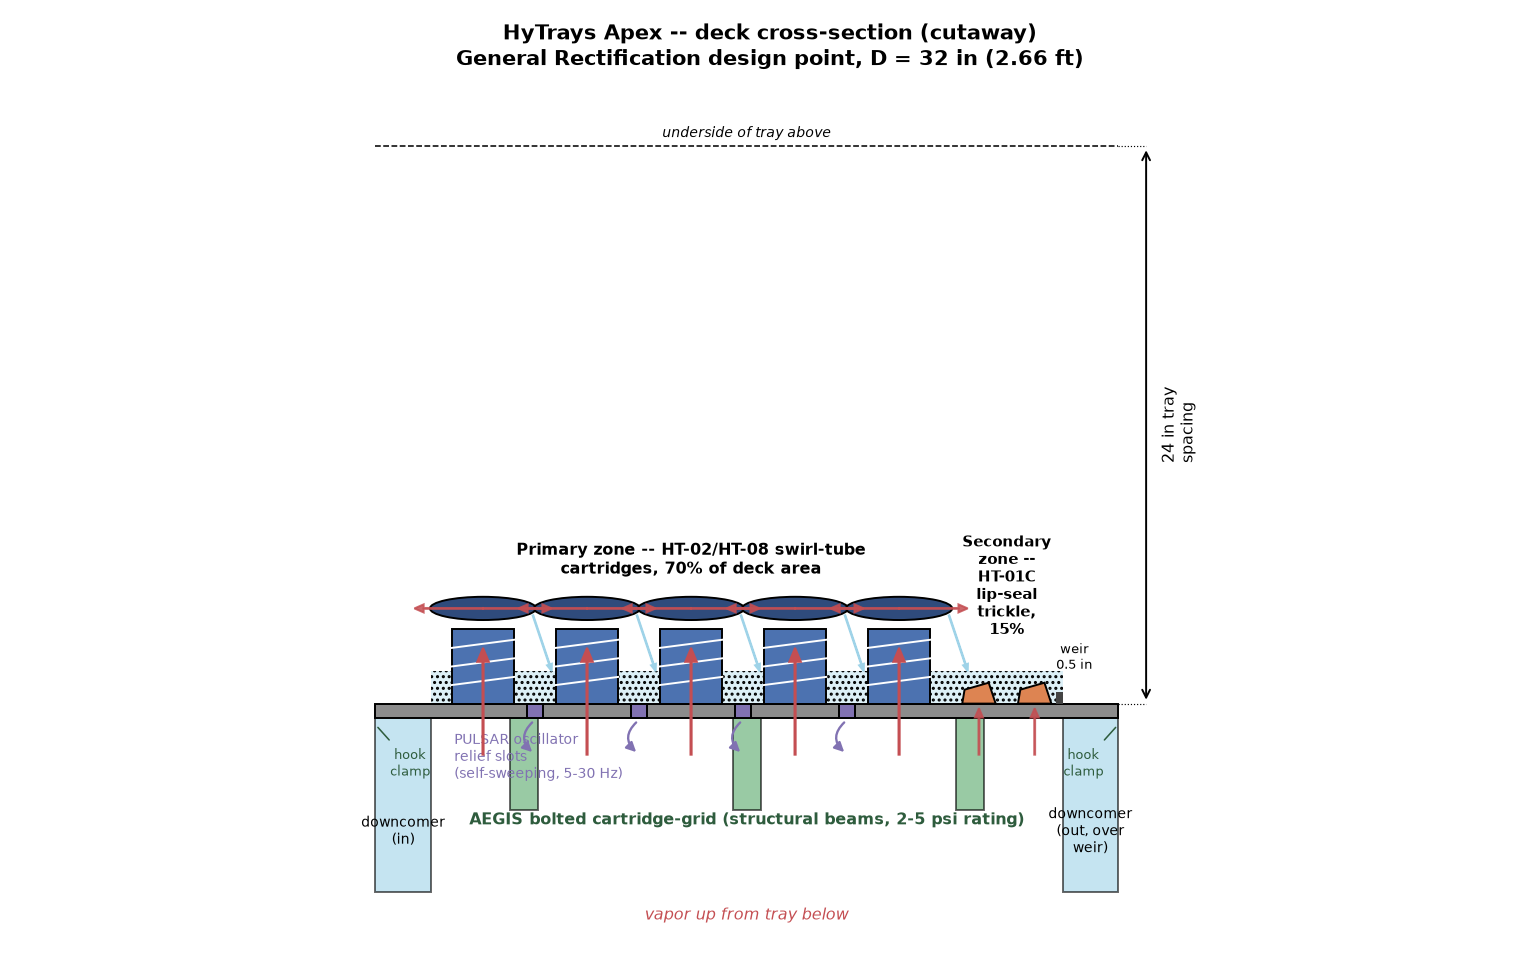
\includegraphics[width=0.88\textwidth]{output/30_apex_cross_section.png}
  \caption{Apex deck cutaway elevation, General Rectification design point
    ($D=\SI{32}{\inch}$, 24-inch tray spacing).  Swirl-tube cartridges (primary
    zone) occupy 70\% of the plan area; LipSeal trickle valves (secondary zone)
    fill the remaining active area adjacent to the downcomers.  PULSAR relief
    slots sit between cartridge footprints; AEGIS structural ribs run beneath
    the deck panels.}
  \label{fig:cross_section}
\end{figure}

\begin{figure}[H]
  \centering
  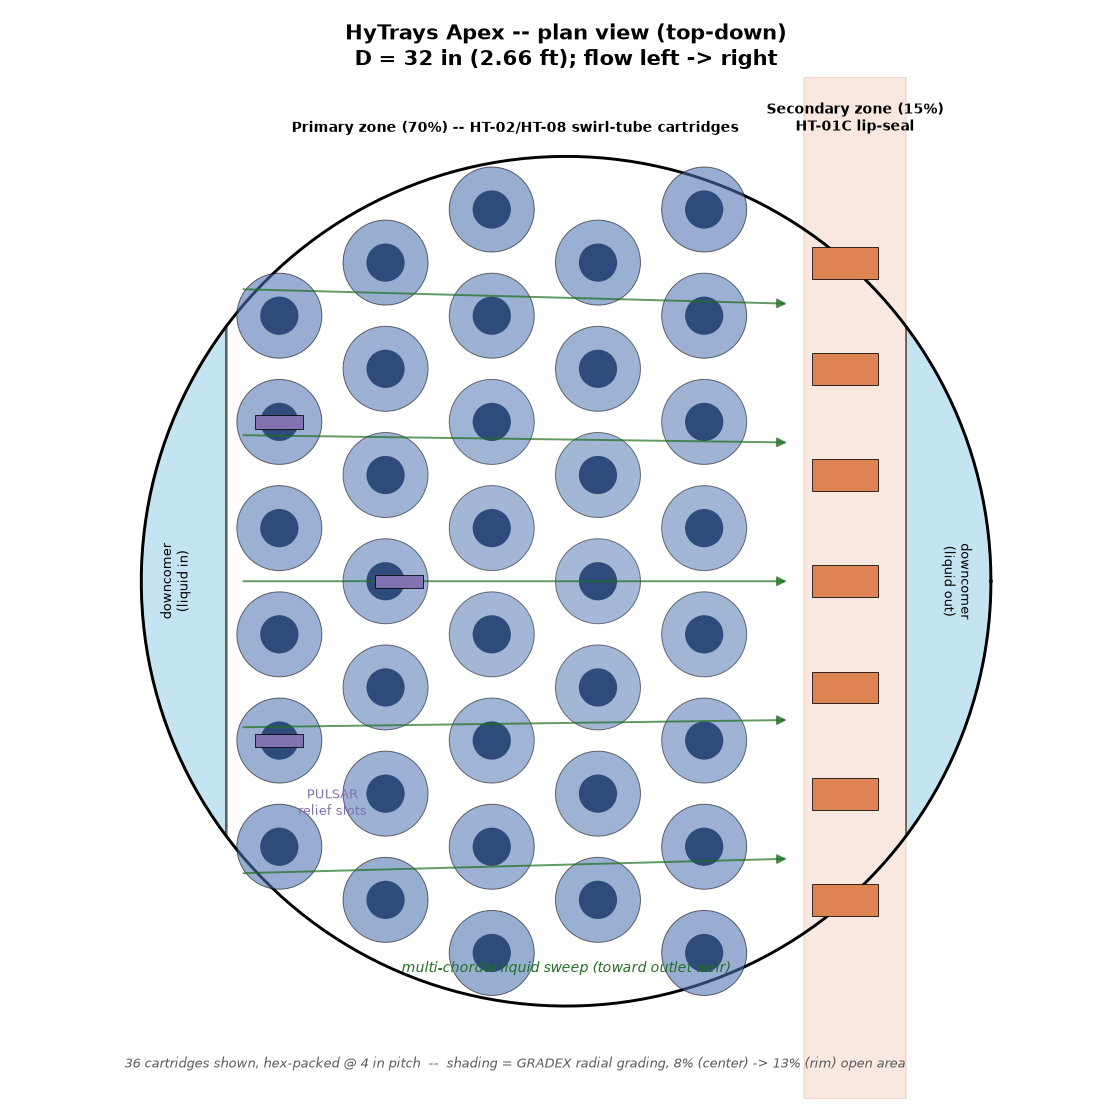
\includegraphics[width=0.72\textwidth]{output/31_apex_plan_view.png}
  \caption{Apex plan view (top-down).  Hex-packed cartridges (circles) in the
    primary zone with GRADEX radial-load shading; LipSeal secondary zone at
    the downcomer edges; downcomers (shaded).}
  \label{fig:plan_view}
\end{figure}

At the General Rectification design point the column is $D = \SI{32}{\inch}$
(2.66\,ft), with a 24-inch tray spacing.  The primary zone contains
approximately 18--22 cartridges of 110\,mm ID on a 155\,mm triangular pitch,
each passing roughly 2.5\,m$^3$/h of liquid and $\SI{25}{m/s}$ slot velocity.
The 0.5-inch outlet weir is the lowest of any tray family evaluated
(sieve: 2.0\,in.; high-performance MD: 1.0\,in.; Ripple: 1.5\,in.),
enabled by the crown-separator mechanical disengagement that removes entrained
liquid before it can be re-entrained by rising vapour.

\subsection{Construction and Manufacturing}
\label{sec:construction}

\paragraph{Swirl-tube cartridges (HT-02/HT-08).}
Fabricated from CF8M (316SS) or Alloy 625 investment castings or CNC-machined
bar stock.  The 6 tangential slots are precision-formed to $\pm$0.1\,mm to
hold the swirl number $S$ within the 1.5--3.0 design band.  The vane crown
(12 vanes at 45$^\circ$) is a separate casting press-fitted and tack-welded to
the tube top.  The HT-08 helical sleeve is machined from 316L bar, coated
with PTFE or DLC to reduce sliding friction.  Each complete cartridge is
factory-tested for slot flow coefficient and sleeve travel before shipment.

\paragraph{Deck panels and AEGIS grid.}
Deck panels are 2.5\,mm 316L stainless, laser-cut with cartridge bores and
PULSAR relief slot locations.  Stiffening ribs (3$\times$20\,mm flat bars,
170\,mm pitch) are TIG-welded to the panel underside.  Hook clamps are
cold-formed from 316L strip, engaged under the factory-welded support ring.
A complete panel with six to eight cartridges weighs approximately 20--28\,kg,
within one-person manway handling limit.

\paragraph{LipSeal valves (HT-01C).}
Stamped 1.5\,mm 316L, with the lip formed by a second progressive die
operation.  No assembly required; valves drop into 70\,mm die-cut deck
holes and are retained by a simple keeper ring.

\paragraph{Lead time and cost drivers.}
The cartridge casting and sleeve machining are the dominant cost and lead-time
items (8--14 weeks from castings; 2--4 weeks from machined bar).  Deck panel
fabrication and hook-clamp assembly add 2--4 weeks.  Repeat-order lead time
shortens significantly once casting dies are amortised.

\subsection{Installation, Maintenance and Cartridge-Swap Procedure}
\label{sec:installation}

\paragraph{Initial installation.}
The AEGIS support ring is welded to the column shell at the tray elevation,
identical to a conventional tray ring (one-time operation, no re-welding in
subsequent turnarounds).  Deck panels are lowered through the manway,
positioned on the support ring and locked by rotating the hook clamps to the
engaged position.  Cartridges are threaded through the panel bores from above
and secured by a quarter-turn bayonet fitting; the LipSeal valves drop in last.
Typical installation time: 4--6\,hours per tray with a two-person crew.

\paragraph{Turnaround maintenance.}
Hook clamps are released, panels lifted out through the manway, and
cartridges withdrawn individually.  Worn or fouled cartridges are replaced
from a spares inventory; the support ring remains in place.  The
cartridge-swap approach means that maintenance cost per tray is dominated by
cartridge replacement rather than shell welding, and that individual stages
can be upgraded independently if a new cartridge design becomes available.

\paragraph{Inspection.}
The crown separator and helical sleeve are accessible for visual inspection
once the cartridge is withdrawn.  Endoscopic inspection of the swirl zone is
possible without cartridge removal.  PULSAR slots and LipSeal valves are
inspectable from above after the cartridges are removed.

% ════════════════════════════════════════════════════════════════════════════
\section{Design Parameter Envelope}
\label{sec:parameters}

Table~\ref{tab:traytype} lists the TrayType parameters for all seven trays
evaluated in the comparison (implemented in \texttt{tray\_library.py}).
Table~\ref{tab:apex_claimband} gives the claimed-band envelope for
Apex-specific parameters, following the format of the HT-0X individual
disclosures.

\begin{table}[H]
\centering
\caption{TrayType parameters for all seven tray families.  ``Capacity factor''
is $k_{\mathrm{cap}}$ in Eq.~\eqref{eq:unf}; ``Efficiency factor'' is $\eta$
in Eq.~\eqref{eq:etray}; ``Turndown'' = $1/f_{\mathrm{min}}$.}
\label{tab:traytype}
\small
\begin{tabular}{lrrrrrrrrrrrr}
\toprule
Tray & $f_{\mathrm{act}}$ & $f_{\mathrm{hole}}$ & $h_w$ (in) & $C_0$
  & $\dpd_{\mathrm{fl}}$ (in) & $\beta$ & $k_{\mathrm{cap}}$ & $\eta$
  & TO & $f_{\mathrm{foul}}$ & $k_{\mathrm{cost}}$\\
\midrule
Sieve              & 0.78 & 0.10 & 2.0 & 0.73 & 0.00 & 0.55 & 1.00 & 1.00 & 2.0:1  & 0.75 & 1.00\\
Dual-Flow          & 1.00 & 0.20 & 0.0 & 0.73 & 0.00 & 0.40 & 1.15 & 0.83 & 1.5:1  & 0.90 & 0.70\\
Moving Valve       & 0.78 & 0.13 & 2.0 & 0.85 & 0.40 & 0.55 & 1.03 & 1.00 & 3.3:1  & 0.70 & 1.35\\
Fixed Valve        & 0.78 & 0.12 & 2.0 & 0.80 & 0.05 & 0.52 & 1.08 & 1.00 & 2.2:1  & 0.85 & 1.20\\
High-Perf.\ MD     & 0.85 & 0.14 & 1.0 & 0.80 & 0.10 & 0.50 & 1.25 & 0.97 & 2.5:1  & 0.75 & 1.55\\
Ripple (Corr.)     & 0.80 & 0.11 & 1.5 & 0.75 & 0.00 & 0.50 & 1.10 & 1.10 & 2.5:1  & 0.72 & 1.15\\
\textbf{Apex}      & \textbf{0.85} & \textbf{0.25} & \textbf{0.5} & \textbf{0.85}
  & \textbf{0.10} & \textbf{0.38} & \textbf{2.50} & \textbf{1.20} & \textbf{22.2:1}
  & \textbf{0.93} & \textbf{3.20}\\
\bottomrule
\end{tabular}
\end{table}

\begin{table}[H]
\centering
\caption{Claim-band table for Apex Trays parameters.  ``Preferred'' values are
the \texttt{APEX} TrayType entry; ranges are dependent-claim fallback positions
informed by the individual HT-0X disclosures.}
\label{tab:apex_claimband}
\small
\begin{tabular}{lcl}
\toprule
Parameter & Claimed band & Preferred\\
\midrule
Active area fraction $f_{\mathrm{active}}$           & 0.80--0.88      & 0.85\\
Hole/slot open area fraction $f_{\mathrm{hole}}$     & 0.20--0.30      & 0.25\\
Outlet weir height $h_{\mathrm{weir}}$               & 0.25--1.0\,in.  & 0.50\,in.\\
Orifice coefficient $C_0$                             & 0.80--0.90      & 0.85\\
Dry-floor dP minimum $\dpd_{\mathrm{floor}}$         & 0.05--0.15\,in. & 0.10\,in.\\
Aeration factor $\beta$                               & 0.30--0.45      & 0.38\\
Capacity factor $k_{\mathrm{cap}}$                   & 1.80--3.00      & 2.50\\
Efficiency factor $\eta$                              & 1.10--1.30      & 1.20\\
Minimum stable load fraction $f_{\mathrm{min}}$      & 0.030--0.070    & 0.045\\
Turndown (= $1/f_{\mathrm{min}}$)                    & 14:1--33:1      & 22.2:1\\
Fouling open-area retention $f_{\mathrm{foul}}$      & 0.88--0.97      & 0.93\\
Relative unit cost factor $k_{\mathrm{cost}}$        & 2.5--4.0        & 3.20\\
Structural uplift rating                              & 2--5\,psi       & 5\,psi\\
Primary zone area fraction                            & 0.65--0.75      & 0.70\\
Secondary zone area fraction                          & 0.10--0.20      & 0.15\\
Swirl-tube ID                                         & 80--150\,mm     & 110\,mm\\
Swirl number $S$                                      & 1.5--3.0        & 2.2\\
Wall acceleration                                     & 30--60\,$g$     & 45\,$g$\\
Tangential slots per cartridge                        & 4--8            & 6\\
Slot exit velocity                                    & 18--35\,m/s     & 25\,m/s\\
Crown vanes / pitch angle                             & 8--16 / 35--55\ensuremath{^\circ}  & 12 / 45\ensuremath{^\circ}\\
AEGIS deck thickness                                  & 2.0--3.0\,mm SS & 2.5\,mm\\
AEGIS rib pitch $s$                                   & $\leq 184$\,mm  & 170\,mm\\
Relief-flap set pressure                              & 1.5--3.0\,psi   & 2.0\,psi\\
\bottomrule
\end{tabular}
\end{table}

% ════════════════════════════════════════════════════════════════════════════
\section{Predicted Performance}
\label{sec:performance}

Table~\ref{tab:genrect} gives the full hydraulics results for the
\textit{General Rectification} service.  Tables~\ref{tab:services} and
\ref{tab:apex_sieve} give the cross-service summary.
All figures are from \texttt{run\_apex\_paper.py}; the design basis is given
in Section~\ref{sec:limitations}.

\begin{table}[H]
\centering
\caption{General Rectification results (T801 basis, 20 theoretical stages).
  All seven tray families sized at $f_{\mathrm{flood}}=0.80$, 24-inch tray
  spacing.  Sieve is the reference ($C_{\mathrm{rel}} = 1.00$).}
\label{tab:genrect}
\small
\begin{tabular}{lrrrrrrrrrr}
\toprule
Tray & $D$ (ft) & $\unf$ (ft/s) & $\dpt$ (psi) & DC (\%)
  & TO & Eff (\%) & $N$ & $H$ (ft) & $\dptot$ (psi) & $C_{\mathrm{rel}}$\\
\midrule
Sieve          & 4.39 & 1.52 & 0.0557 & 34 & 2.0:1  & 76.2  & 27 & 64.0 & 1.503 & 1.00\\
Dual-Flow      & 3.61 & 1.75 & 0.0170 & n/a& 1.5:1  & 63.2  & 32 & 74.0 & 0.543 & 0.84\\
Moving Valve   & 4.32 & 1.56 & 0.0395 & 27 & 3.3:1  & 76.2  & 27 & 64.0 & 1.065 & 1.08\\
Fixed Valve    & 4.22 & 1.64 & 0.0446 & 30 & 2.2:1  & 76.2  & 27 & 64.0 & 1.204 & 1.01\\
High-Perf.\ MD & 3.76 & 1.90 & 0.0351 & 23 & 2.5:1  & 73.9  & 28 & 66.0 & 0.983 & 0.97\\
Ripple (Corr.) & 4.13 & 1.67 & 0.0477 & 30 & 2.5:1  & 83.8  & 24 & 58.0 & 1.144 & 0.87\\
\textbf{Apex}  & \textbf{2.66} & \textbf{3.79} & \textbf{0.0317} & \textbf{23}
  & \textbf{22.2:1} & \textbf{91.4} & \textbf{22} & \textbf{54.0}
  & \textbf{0.697} & \textbf{0.64}\\
\bottomrule
\end{tabular}
\end{table}

\begin{figure}[H]
  \centering
  \begin{subfigure}[t]{0.49\textwidth}
    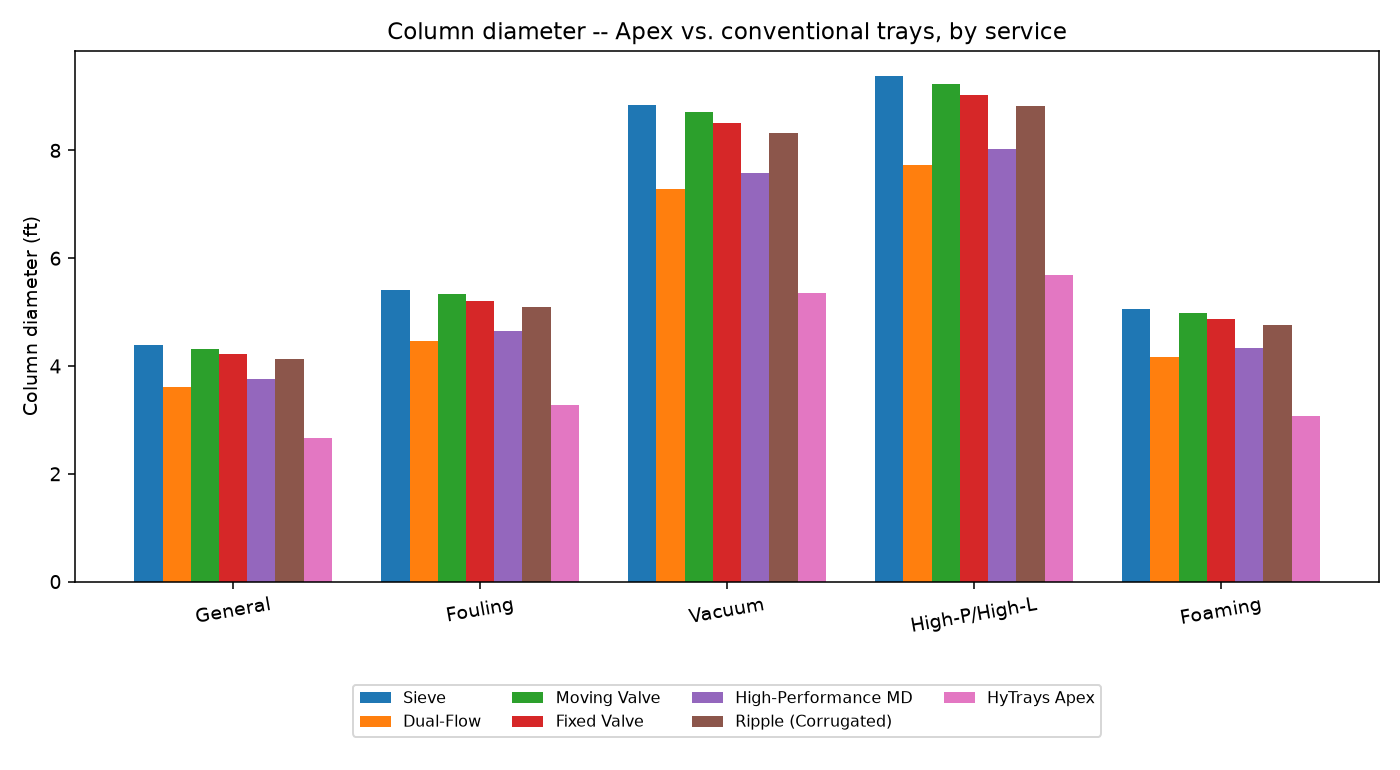
\includegraphics[width=\linewidth]{output/21_apex_diameter_by_service.png}
    \caption{Column diameter.}
    \label{fig:diameter}
  \end{subfigure}
  \hfill
  \begin{subfigure}[t]{0.49\textwidth}
    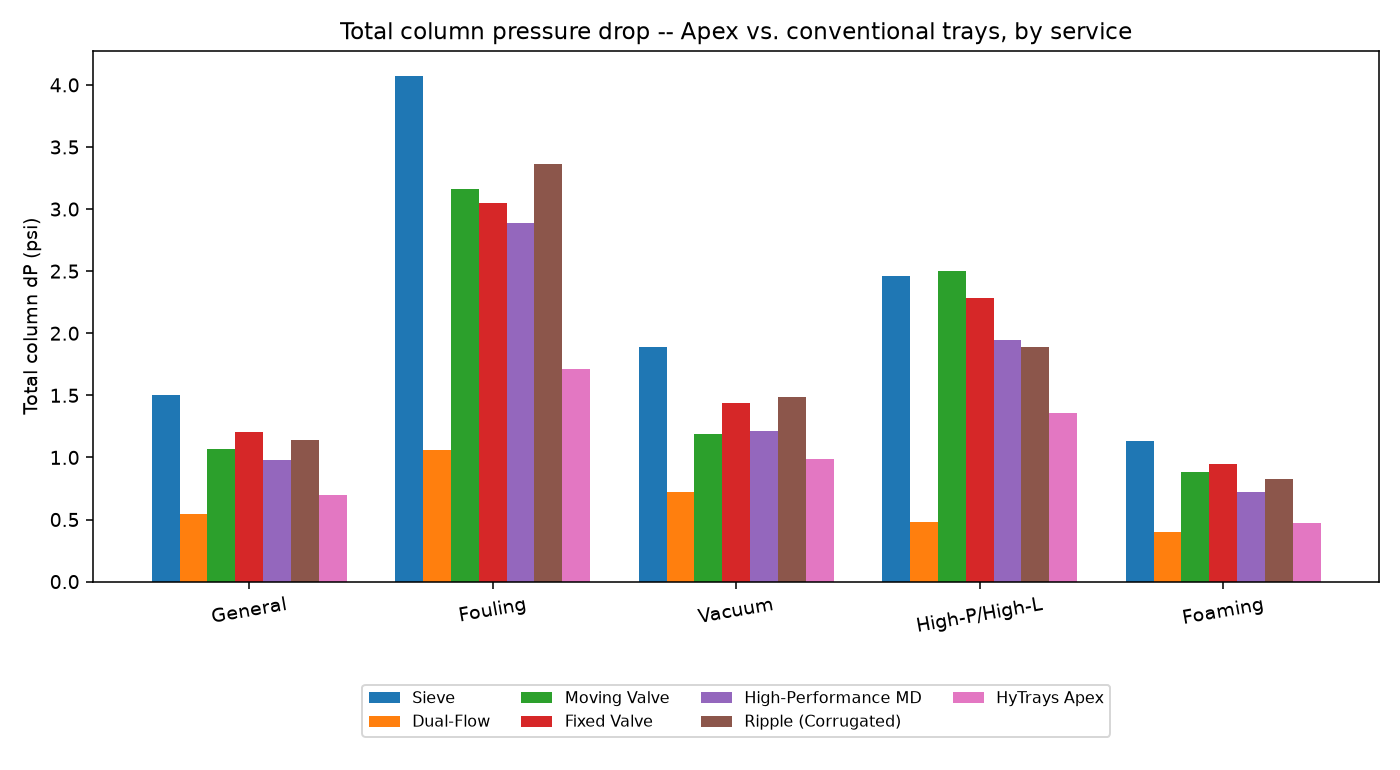
\includegraphics[width=\linewidth]{output/22_apex_total_dp_by_service.png}
    \caption{Total column pressure drop.}
    \label{fig:dp}
  \end{subfigure}
  \caption{Predicted column diameter and total pressure drop for all seven
    tray families across five services.}
  \label{fig:service_plots_1}
\end{figure}

\begin{figure}[H]
  \centering
  \begin{subfigure}[t]{0.49\textwidth}
    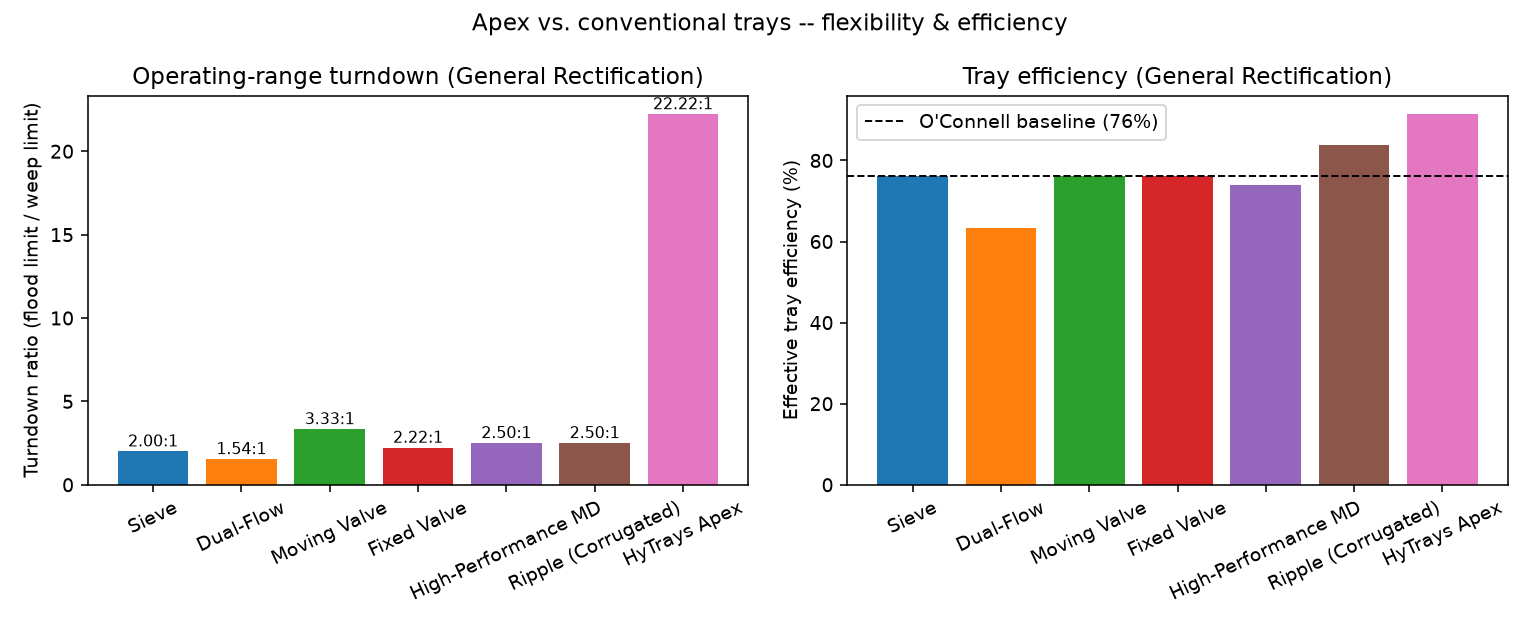
\includegraphics[width=\linewidth]{output/23_apex_turndown_and_efficiency.png}
    \caption{Turndown ratio and tray efficiency (General Rectification).}
    \label{fig:to_eff}
  \end{subfigure}
  \hfill
  \begin{subfigure}[t]{0.49\textwidth}
    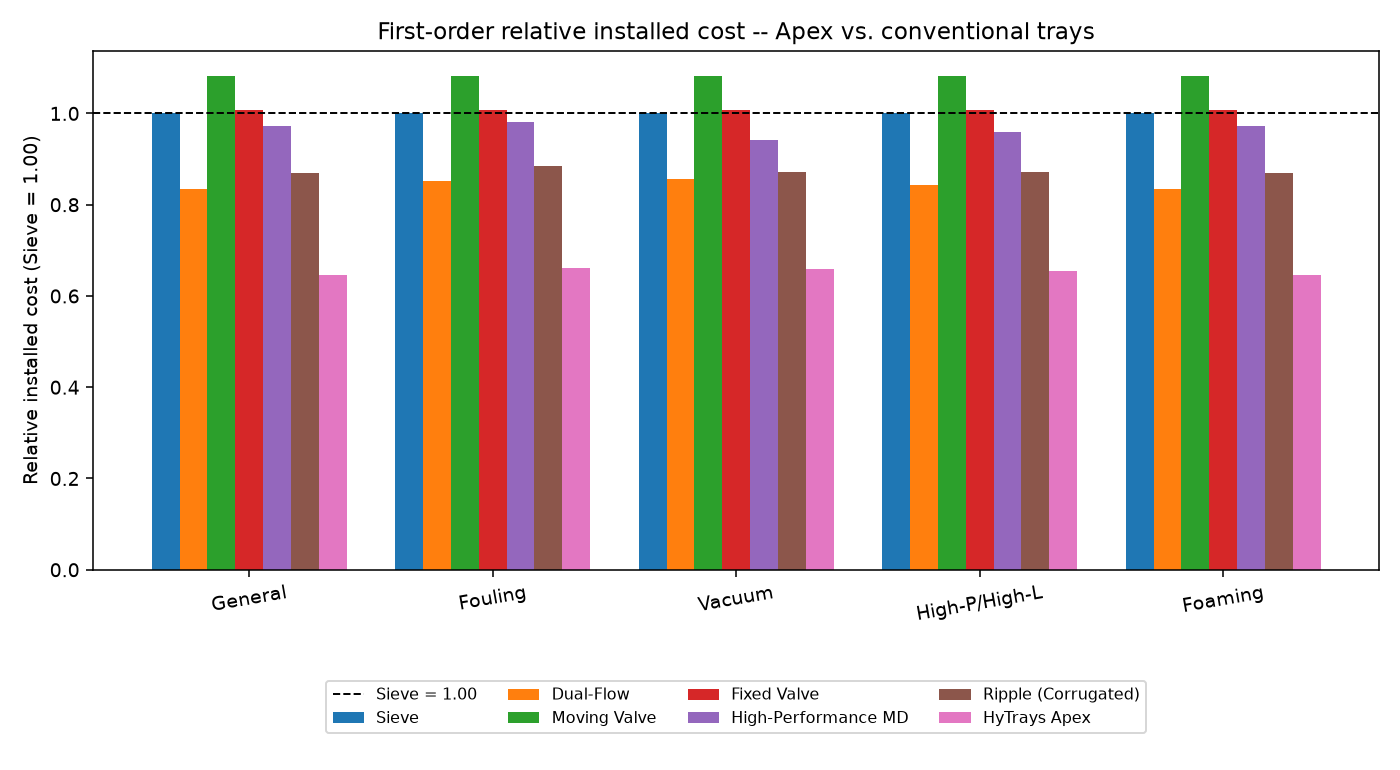
\includegraphics[width=\linewidth]{output/24_apex_relative_cost_by_service.png}
    \caption{Relative installed cost vs.\ sieve = 1.00.}
    \label{fig:cost}
  \end{subfigure}
  \caption{Predicted operating range and cost for all seven tray families.}
  \label{fig:service_plots_2}
\end{figure}

\begin{table}[H]
\centering
\caption{Apex predicted performance across five services ($N_{\mathrm{th}}=20$,
  $H_S=24$\,in.).  Sieve results shown alongside for direct comparison.}
\label{tab:services}
\small
\begin{tabular}{llrrrrrrrr}
\toprule
Service & Tray & $D$ (ft) & $\dpt$ (psi) & DC (\%) & TO & Eff (\%)
  & $N$ & $\dptot$ (psi) & $C_{\mathrm{rel}}$\\
\midrule
\multirow{2}{*}{General}
  & Sieve          & 4.39 & 0.056 & 34 & 2.0:1  & 76.2 & 27 & 1.503 & 1.00\\
  & \textbf{Apex}  & \textbf{2.66} & \textbf{0.032} & \textbf{23} & \textbf{22.2:1}
    & \textbf{91.4} & \textbf{22} & \textbf{0.697} & \textbf{0.64}\\
\midrule
\multirow{2}{*}{Fouling}
  & Sieve          & 5.42 & 0.091 & 41 & 2.0:1  & 33.5 & 45 & 4.070 & 1.00\\
  & \textbf{Apex}  & \textbf{3.28} & \textbf{0.045} & \textbf{33} & \textbf{22.2:1}
    & \textbf{40.2} & \textbf{38} & \textbf{1.711} & \textbf{0.66}\\
\midrule
\multirow{2}{*}{Vacuum}
  & Sieve          & 8.84 & 0.105 & 37 & 2.0:1  & 45.9 & 18 & 1.891 & 1.00\\
  & \textbf{Apex}  & \textbf{5.35} & \textbf{0.066} & \textbf{26} & \textbf{22.2:1}
    & \textbf{55.0} & \textbf{15} & \textbf{0.985} & \textbf{0.66}\\
\midrule
\multirow{2}{*}{High-P/High-L}
  & Sieve          & 9.38 & 0.051 & 43 & 2.0:1  & 84.7 & 48 & 2.463 & 1.00\\
  & \textbf{Apex}  & \textbf{5.68} & \textbf{0.034} & \textbf{54} & \textbf{22.2:1}
    & \textbf{100.0} & \textbf{40} & \textbf{1.361} & \textbf{0.65}\\
\midrule
\multirow{2}{*}{Foaming}
  & Sieve          & 5.07 & 0.042 & 28 & 2.0:1  & 76.2 & 27 & 1.130 & 1.00\\
  & \textbf{Apex}  & \textbf{3.07} & \textbf{0.021} & \textbf{17} & \textbf{22.2:1}
    & \textbf{91.4} & \textbf{22} & \textbf{0.470} & \textbf{0.64}\\
\bottomrule
\end{tabular}
\end{table}

\begin{table}[H]
\centering
\caption{Apex vs.\ sieve: diameter and total pressure-drop changes across
  five services.  Changes are computed from model output and reflect the
  theoretical performance of the TrayType parameter set; they do not
  account for column-specific layout or nozzle constraints.}
\label{tab:apex_sieve}
\small
\begin{tabular}{lrrrrrr}
\toprule
Service & $D_{\mathrm{Sieve}}$ (ft) & $D_{\mathrm{Apex}}$ (ft) & $\Delta D$
  & $\dptot_{\mathrm{Sieve}}$ (psi) & $\dptot_{\mathrm{Apex}}$ (psi) & $\Delta\dptot$\\
\midrule
General      & 4.39 & 2.66 & $-39\%$ & 1.503 & 0.697 & $-54\%$\\
Fouling      & 5.42 & 3.28 & $-39\%$ & 4.070 & 1.711 & $-58\%$\\
Vacuum       & 8.84 & 5.35 & $-39\%$ & 1.891 & 0.985 & $-48\%$\\
High-P/High-L& 9.38 & 5.68 & $-39\%$ & 2.463 & 1.361 & $-45\%$\\
Foaming      & 5.07 & 3.07 & $-39\%$ & 1.130 & 0.470 & $-58\%$\\
\bottomrule
\end{tabular}
\end{table}

\paragraph{Note on the uniform diameter reduction.}
The 39\% reduction is identical across all services because it derives solely
from Equation~\eqref{eq:dratio}: $k_{\mathrm{cap}}$ and $f_{\mathrm{active}}$
are TrayType constants, not functions of the service properties.  The
pressure-drop reduction varies by service because the wet-tray pressure drop
(Eq.~\eqref{eq:dptray_psi}) depends on $\rho_L$, $h_{\mathrm{weir}}$,
$\hcl$, and $\beta$, all of which change with service.

% ════════════════════════════════════════════════════════════════════════════
\section{Fouling Sensitivity}
\label{sec:fouling}

\begin{table}[H]
\centering
\caption{Fouling sensitivity: effective open-area retention and dry-tray pressure
  drop increase when fully fouled.  Computed flow-independently as
  $\dpd_{\mathrm{fouled}}/\dpd_{\mathrm{clean}} = (f_{\mathrm{hole}}/f_{\mathrm{hole,eff}})^2$
  $= 1/f_{\mathrm{foul}}^2$.}
\label{tab:fouling}
\small
\begin{tabular}{lcc}
\toprule
Tray & Open-area retention $f_{\mathrm{foul}}$ & Dry-tray $\dpd$ increase\\
\midrule
Sieve              & 0.75 & $+78\%$\\
Dual-Flow          & 0.90 & $+23\%$\\
Moving Valve       & 0.70 & $+104\%$\\
Fixed Valve        & 0.85 & $+38\%$\\
High-Perf.\ MD     & 0.75 & $+78\%$\\
Ripple (Corr.)     & 0.72 & $+93\%$\\
\textbf{Apex}      & \textbf{0.93} & $\boldsymbol{+16\%}$\\
\bottomrule
\end{tabular}
\end{table}

\begin{figure}[H]
  \centering
  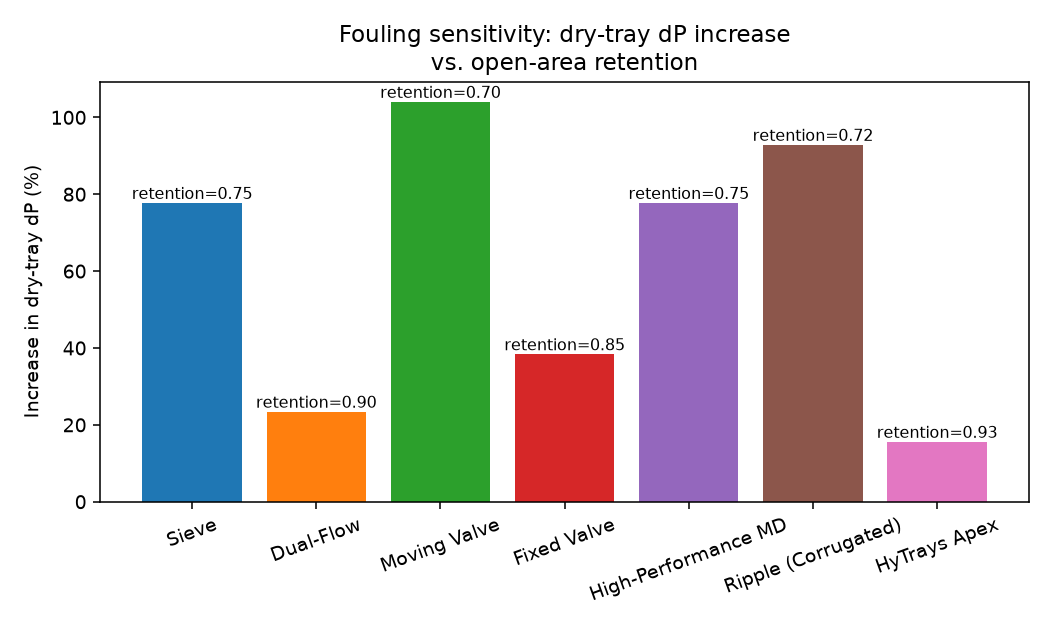
\includegraphics[width=0.72\textwidth]{output/25_apex_fouling_sensitivity.png}
  \caption{Dry-tray pressure drop increase vs.\ open-area retention under
    fouling conditions.  Apex's 93\% retention is the highest in the comparison
    family, predicting the smallest fouling penalty ($+$16\%).}
  \label{fig:fouling}
\end{figure}

% ════════════════════════════════════════════════════════════════════════════
\section{Cost Analysis}
\label{sec:costanalysis}

Table~\ref{tab:cost} gives the first-order relative installed cost breakdown
for the General Rectification case, following Equations~\eqref{eq:shellproxy}--\eqref{eq:crel}.

\begin{table}[H]
\centering
\caption{First-order relative installed cost breakdown, General Rectification.
  Sieve = 1.00.  Shell proxy = $D\times H$; tray proxy = $D^2\times N\times k_{\mathrm{cost}}$.
  Weights: shell 70\%, trays 30\%.}
\label{tab:cost}
\small
\begin{tabular}{lrrr}
\toprule
Tray & Shell proxy ratio & Tray-hardware proxy ratio & $C_{\mathrm{rel}}$\\
\midrule
Sieve              & 1.00 & 1.00 & 1.00\\
Dual-Flow          & 0.95 & 0.56 & 0.84\\
Moving Valve       & 0.99 & 1.31 & 1.08\\
Fixed Valve        & 0.96 & 1.11 & 1.01\\
High-Perf.\ MD     & 0.88 & 1.18 & 0.97\\
Ripple (Corr.)     & 0.85 & 0.91 & 0.87\\
\textbf{Apex}      & \textbf{0.51} & \textbf{0.96} & \textbf{0.64}\\
\bottomrule
\end{tabular}
\end{table}

\paragraph{Interpretation.}
Apex's tray-hardware proxy (0.96) is nearly equal to sieve (1.00) despite
$k_{\mathrm{cost}} = 3.20$, because the smaller diameter and lower actual
tray count ($N=22$ vs.\ 27) reduce the $D^2\times N$ product enough to
offset the 3.2$\times$ unit cost.  The dominant saving comes from the shell
proxy (0.51): the 39\% diameter reduction cuts $D$ by a factor of 0.606,
and the reduced tray count cuts $H$ by a factor of $54/64 = 0.844$, giving
a shell-proxy reduction of $0.606\times0.844 = 0.511$.  The 70\% shell
weight then produces most of the total cost saving.

This model does not capture: detailed vessel design (nozzles, manways,
platforms), foundation and plot costs, process-piping re-work if the
diameter changes from an existing design, or the higher installed cost of
precision cartridges relative to standard internals in a retrofit.

% ════════════════════════════════════════════════════════════════════════════
\section{Technical Comparison with Conventional Tray Families}
\label{sec:comparison}

\begin{figure}[H]
  \centering
  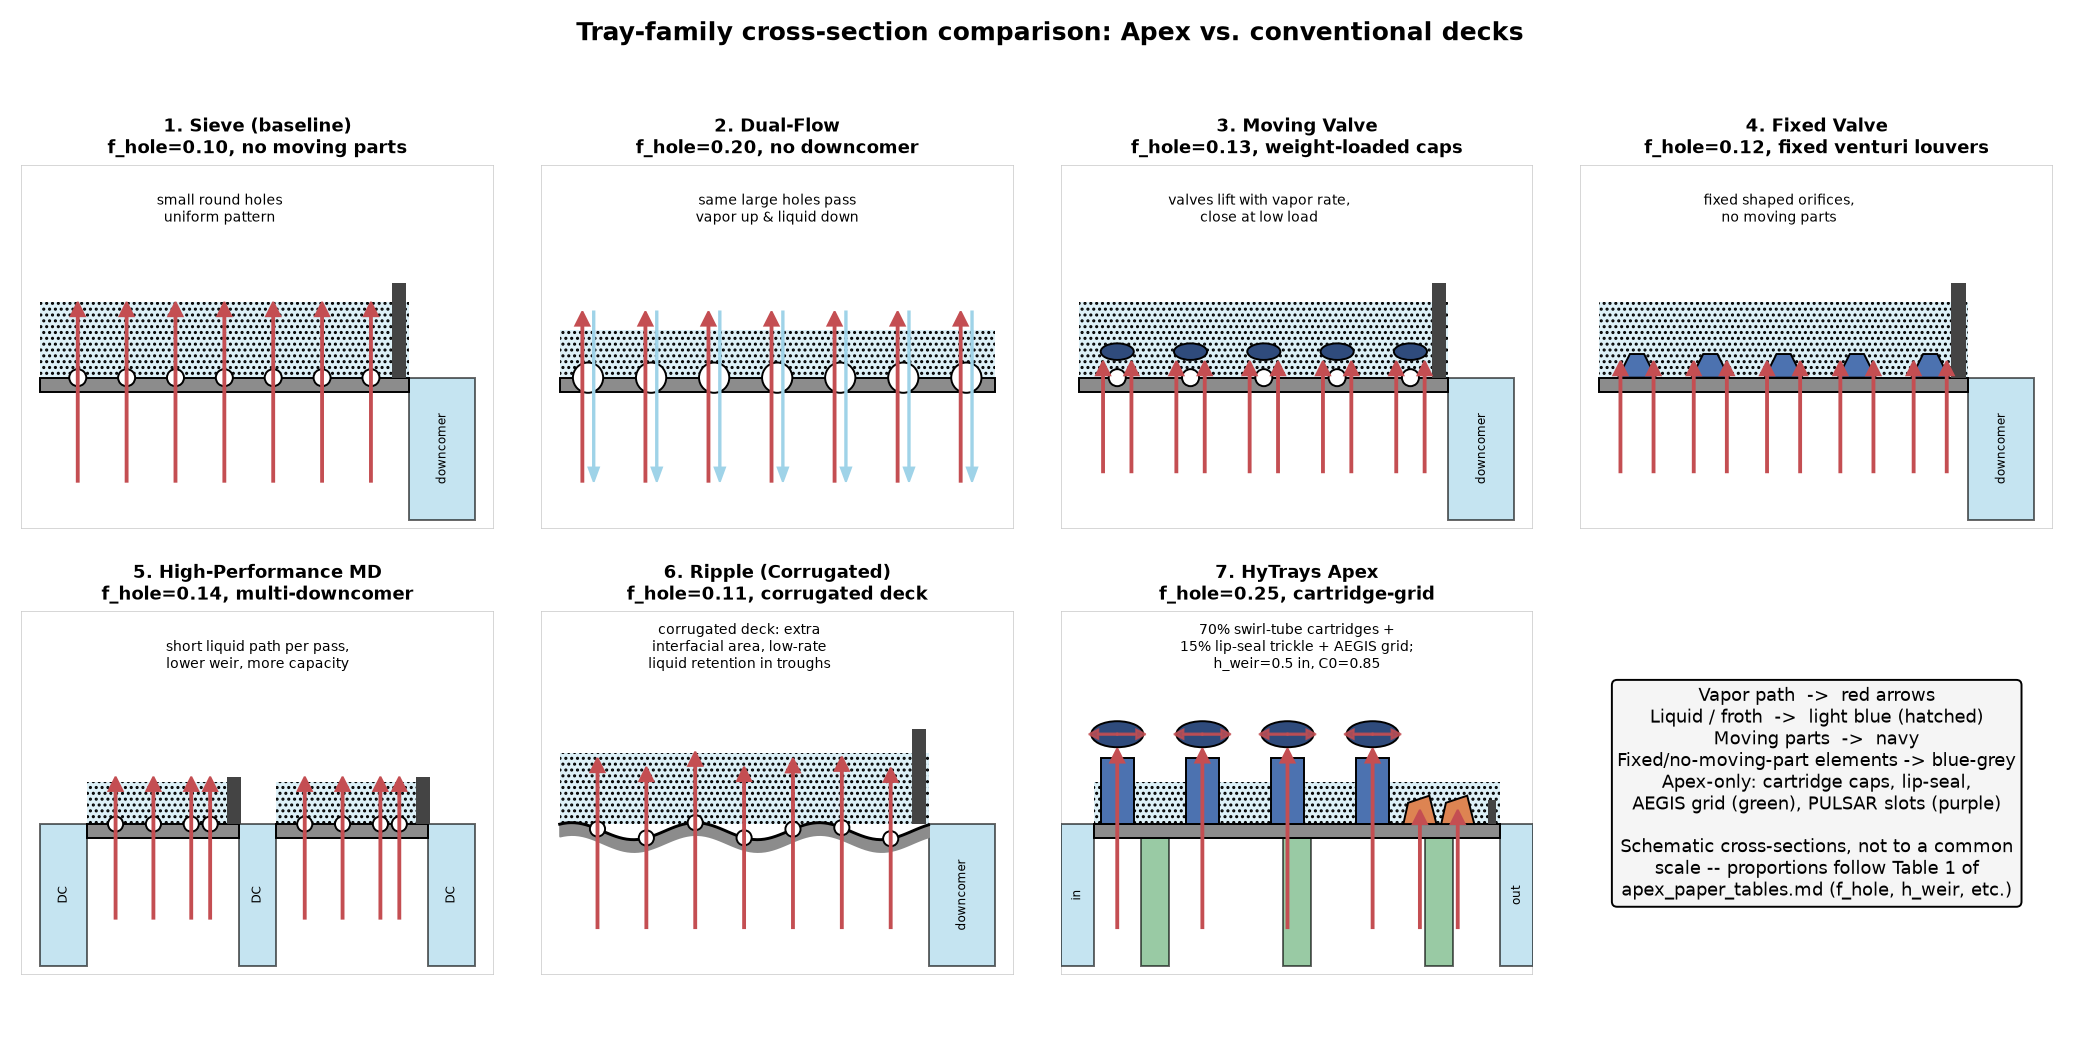
\includegraphics[width=\textwidth]{output/32_tray_family_cross_sections.png}
  \caption{Cross-section schematic comparison of all seven tray families
    evaluated.  Left to right: Sieve, Dual-Flow, Moving Valve, Fixed Valve,
    High-Performance Multi-Downcomer, Ripple (Corrugated), Apex Trays.}
  \label{fig:family_cross_sections}
\end{figure}

Table~\ref{tab:comparison} summarises the relative standing of each tray
family across the key discriminators used in tray-selection practice
(following Kister, \textit{Distillation Design}, Ch.~1).  Ratings are based
solely on the model predictions in Tables~\ref{tab:traytype}--\ref{tab:cost};
qualitative assessments are noted where the model does not directly compute
the relevant quantity.

\begin{table}[H]
\centering
\caption{Comparative assessment of the seven tray families across key
  selection discriminators (General Rectification basis unless noted;
  $\uparrow$ = better, $\downarrow$ = worse, relative to sieve).}
\label{tab:comparison}
\small
\begin{tabular}{lccccccc}
\toprule
 & Sieve & Dual-Flow & Mv.~Valve & Fx.~Valve & Hi-Perf.~MD & Ripple & Apex\\
\midrule
Vapour capacity             & base & $\uparrow$ & $\approx$ & $\uparrow$ & $\uparrow$  & $\uparrow$ & $\uparrow\uparrow$\\
Liquid capacity             & base & n/a  & $\approx$ & $\approx$ & $\uparrow$  & $\approx$ & $\approx$\\
Turndown ratio              & 2.0:1& 1.5:1& 3.3:1 & 2.2:1 & 2.5:1  & 2.5:1 & 22.2:1\\
Tray efficiency             & 76\% & 63\% & 76\%  & 76\%  & 74\%   & 84\%  & 91\%\\
Wet-tray dP (psi)           & 0.056& 0.017& 0.040 & 0.045 & 0.035  & 0.048 & 0.032\\
Fouling resistance          & base & $\uparrow$ & $\downarrow$ & $\approx$ & base & $\downarrow$ & $\uparrow\uparrow$\\
Moving parts                & none & none & yes   & none  & limited& none  & sleeve\\
Downcomer required          & yes  & no   & yes   & yes   & yes    & yes   & yes\\
Structural uplift           & low  & low  & low   & low   & mod.   & low   & 2--5\,psi\\
Rel.\ installed cost (Gen.) & 1.00 & 0.84 & 1.08  & 1.01  & 0.97   & 0.87  & 0.64\\
Fabrication complexity      & low  & low  & mod.  & low   & mod.   & mod.  & high\\
\bottomrule
\end{tabular}
\end{table}

\paragraph{Capacity.}
Apex's capacity factor (2.50) is the highest in the comparison, predicting
the smallest column diameter at every service.  The next highest is
High-Performance MD (1.25), followed by Dual-Flow (1.15).  The capacity
advantage is structural: the swirl-tube centrifugal mechanism bypasses the
gravity-settling Souders-Brown limit that governs all other trays evaluated.

\paragraph{Turndown.}
Apex's predicted 22.2:1 turndown is substantially larger than all other
families, which range from 1.5:1 (Dual-Flow) to 3.3:1 (Moving Valve).  This
derives entirely from $f_{\mathrm{min}} = 0.045$ assigned to the two-zone
mechanism; as noted in Section~\ref{sec:limitations}, this is the most
uncertain parameter in the model.

\paragraph{Efficiency.}
O'Connell baseline at the General Rectification conditions gives 76.2\%.
Apex's efficiency factor of 1.20 raises this to 91.4\%; Ripple at 1.10 gives
83.8\%; all others are at or below the sieve baseline of 76.2\%.  The
efficiency uplift reduces $N_{\mathrm{actual}}$ from 27 (sieve) to 22 (Apex),
contributing to the column height and cost reductions.

\paragraph{Pressure drop.}
Apex at 0.032\,psi/tray and 0.697\,psi total is the second-lowest after
Dual-Flow (0.017\,psi/tray, 0.543\,psi total), and the lowest among trays
with a downcomer.  The low $\dpt$ comes from the combination of low $\beta$
(0.38), low $h_{\mathrm{weir}}$ (0.5\,in.), high $f_{\mathrm{hole}}$ (0.25)
and fewer actual trays ($N = 22$).

\paragraph{Fouling resistance.}
Moving Valve and Ripple have the lowest open-area retention under fouling
(0.70 and 0.72), predicting $+$104\% and $+$93\% dry-tray dP increases.
Dual-Flow is the best of the conventional designs at 0.90 ($+$23\%), followed
by Fixed Valve (0.85, $+$38\%).  Apex at 0.93 ($+$16\%) is the highest,
reflecting PULSAR self-sweeping and the large-slot geometry.

\paragraph{Fabrication and cost.}
Apex's relative unit cost factor of 3.20 is the highest (precision
investment-cast cartridges plus helical sleeves plus AEGIS grid assembly).
However, the installed cost is the lowest (0.64) because the shell dominates
and Apex's smaller diameter reduces shell cost by $\approx$49\%.

% ════════════════════════════════════════════════════════════════════════════
\section{Claims (Draft)}
\label{sec:claims}

\textbf{Claim 1.}
A vapour--liquid contacting tray comprising a structural cartridge-grid
framework and an active deck panel, the active deck divided into a primary
contacting zone ($\geq 60\%$ of the column cross-sectional area) comprising
an array of axial swirl-tube cartridges, and a secondary contacting zone
(10--20\% of the column cross-sectional area) comprising lip-sealed dual-flow
trickle valves, wherein the primary zone operates at a flooding capacity
factor $k_{\mathrm{cap}} \geq 1.8$ relative to the Fair sieve baseline at
equal tray spacing, and the secondary zone sustains vapour--liquid contact
at vapour loads below 10\% of the primary-zone design basis.

\textbf{Claim 2.}
The tray of Claim 1, wherein the swirl-tube cartridges each comprise
tangential vapour-inlet slots (4--8 per tube), liquid-metering ports feeding
from the deck pool below the slots, and a vane crown separator at the tube
exit that discharges separated liquid into a collection annulus draining to
the outlet-weir region of the same tray.

\textbf{Claim 3.}
The tray of Claim 2, wherein the tangential slots are formed in a
back-drivable helical sleeve that passively opens slot area with increasing
vapour momentum, and the sleeve reverts to a fixed-geometry open position if
mechanically seized.

\textbf{Claim 4.}
The tray of Claim 1, wherein self-sweeping oscillator relief slots are
located in the deck plate between cartridge footprints, each slot held closed
by a spring or weight-loaded cap that opens momentarily when the
deck differential pressure exceeds a set threshold and reseats thereafter.

\textbf{Claim 5.}
The tray of Claim 1, wherein a variable-pitch cartridge layout and
multi-chordal liquid-path baffles are applied across the primary zone to
equalize the local vapour--liquid ratio, targeting a tray efficiency factor
$\eta \geq 1.10$ above the O'Connell single-value baseline.

\textbf{Claim 6.}
The tray of Claim 1, wherein the structural cartridge-grid comprises a
welded support ring, deck panels locked to the ring by interlocking hook
clamps, stiffening ribs at pitch $s \leq t\sqrt{\sigma_{\mathrm{allow}}/(0.75\,q)}$,
and integral relief flaps, providing a structural vapour-uplift rating of at
least 21\,kPa (3\,psi) without reducing active bubbling area by more than 5\%.

\textbf{Claim 7.}
The tray of Claim 6, wherein the cartridges are individually removable
through a column manway and replaceable without modification to the support
ring or column shell.

\textbf{Claim 8.}
The tray of Claim 1, having an active-area fraction $f_{\mathrm{active}}$ of
0.80--0.88, an open-area fraction $f_{\mathrm{hole}}$ of 0.20--0.30, and an
outlet weir height of 0.25--1.0\,inch.

\textbf{Claim 9.}
A column containing trays according to any preceding claim.

\textbf{Claim 10.}
A method of revamping a distillation column comprising replacing existing
cross-flow trays with trays according to Claim 1 at equal or reduced tray
spacing, thereby reducing column diameter requirements by at least 30\%
relative to a sieve tray sized on the same service basis.

% ════════════════════════════════════════════════════════════════════════════
\section{Industrial Applicability}
\label{sec:applicability}

\paragraph{Capacity-constrained columns.}
The predicted 39\% diameter reduction makes Apex applicable to
shell-limited revamp situations where increasing throughput within an existing
shell is the primary objective: C$_3$ splitters, demethanisers, FCC main
fractionator top sections, and offshore columns where shell dimensions are
fixed by deck loading or existing foundations.

\paragraph{Wide-range operating columns.}
The predicted 22.2:1 turndown makes Apex applicable to columns that must
follow variable-rate feedstocks or operate at deep turndown without dumping:
batch-integrated continuous columns, swing-service units, and
grade-change-intensive operations.

\paragraph{Fouling and heavy-ends services.}
The 93\% open-area retention under fouling and the PULSAR self-sweeping
mechanism make Apex applicable to vacuum residue and atmospheric
heavy-ends services where conventional trays foul within one run.  The
cartridge-swap maintenance procedure also reduces turnaround duration when
complete tray replacement is needed.

\paragraph{Energy-intensive separations.}
The 54\% reduction in total column pressure drop (General Rectification basis)
reduces the reboiler duty at the base and condenser duty at the top, with a
corresponding reduction in energy consumption per unit of separation.  The
efficiency improvement ($+15$ percentage points) reduces actual tray count
and column height, providing capital savings and potentially allowing
additional theoretical stages within the existing shell height.

\paragraph{Prior-art neighbours to clear.}
Shell ConSep/swirl-tube art and continuations; Koch-Glitsch SUPERFRAC and UFM
multi-downcomer patents; lip-valve and check-valve tray art (Nutter, Koch,
Sulzer); structural hold-down and bolt-down tray art; GRADEX/multi-chordal
tray grading art (if separately patented); self-sweeping oscillator valve art.
The asserted inventive step is the \textit{integrated} architecture: pairing
the primary swirl-tube zone with a dedicated secondary trickle zone for
turndown, laying radial-grading and self-sweeping treatments over both, and
mounting the result on a structural grid rated for 2--5\,psi uplift, all in
a single bolt-in deck.

% ════════════════════════════════════════════════════════════════════════════
\section{Limitations and Model Caveats}
\label{sec:limitations}

\begin{enumerate}[nosep]
  \item \textbf{One-dimensional model.}
    The hydraulics engine (\texttt{column\_hydraulics.py}) is a 1-D correlation
    framework.  It cannot resolve the radial or azimuthal vapour/liquid
    distribution within a tray, the coupled behaviour of the two contacting
    zones, or the unsteady aerodynamics of the swirl-tube cartridges.  The
    TrayType parameter set (\texttt{APEX}) is a parameterisation of the
    expected behaviour, not a simulation of the physical mechanism.

  \item \textbf{Capacity factor ($k_{\mathrm{cap}} = 2.50$).}
    This is the most influential single parameter (it controls all
    diameter results via Eq.~\eqref{eq:dratio}).  It is derived from
    swirl-tube droplet-trajectory analysis and scaling arguments
    (Section~\ref{sec:primary}), not from tray-scale measurements.
    Cold-flow and hot-rig confirmation is required before this value can
    be used in a final design.

  \item \textbf{Minimum stable load fraction ($f_{\mathrm{min}} = 0.045$).}
    This determines the 22.2:1 turndown claim and cannot be derived from a
    1-D model.  The two-zone mechanism (Section~\ref{sec:secondary}) is the
    proposed physical basis; its validity depends on LipSeal lip-seating
    performance, sleeve-closure behaviour at low vapour rate, and absence of
    maldistribution between the two zones across the tray area.

  \item \textbf{Service properties.}
    The General Rectification case is anchored to T801 stream data from
    \texttt{Hydraulics/HMB.xlsx}; liquid density, viscosity, surface tension
    and relative volatility are engineering estimates.  The remaining four
    services use representative property sets.  Substituting rigorous
    simulator-derived tray-level properties will shift all results.

  \item \textbf{Cost model.}
    The two-proxy cost model (Section~\ref{sec:cost}) is a screening tool,
    not an engineering estimate.  It does not capture: detailed vessel
    mechanical design (nozzle re-rating, foundation loading), plot
    re-configuration, process-piping modifications, AEGIS welded-ring
    installation cost (one-time), cartridge procurement lead time, or
    vendor-specific fabrication pricing.

  \item \textbf{Downcomer backup at High-P/High-L service.}
    Table~\ref{tab:services} shows Apex at 54\% downcomer backup for the
    High-Pressure/High-Liquid-Load service.  Although within the 100\% limit,
    this is the highest Apex figure across all services; detailed downcomer
    sizing with actual tray-level liquid loads should be conducted.

  \item \textbf{Physical mechanisms not modelled.}
    The model does not capture: PULSAR slot cycling dynamics, GRADEX-driven
    local vapour/liquid equalisation, HT-08 sleeve response lag, or the
    interaction between the crown-separator liquid annulus and the deck pool
    at off-design vapour rates.
\end{enumerate}

% ════════════════════════════════════════════════════════════════════════════
\section{References and File Index}
\label{sec:refs}

\paragraph{Hydraulics correlations.}
\begin{itemize}[nosep]
  \item Fair, J.R., ``How to Predict Sieve Tray Entrainment and Flooding,''
    \textit{Petro/Chem Engineer}, 1961.  [Capacity $\Csb$ correlation.]
  \item Kister, H.Z., \textit{Distillation Design}, McGraw-Hill, 1992, Ch.~6.
    [Dry-tray orifice equation, Francis weir, downcomer apron loss, tray
    selection guidance.]
  \item O'Connell, H.E., ``Plate Efficiency of Fractionating Columns and
    Absorbers,'' \textit{Trans.\ AIChE} 42 (1946).  [Overall column
    efficiency $\eoc$.]
  \item Towler, G.P.\ and Sinnott, R.K., \textit{Chemical Engineering Design},
    2nd ed., Elsevier, 2013.  [Cost model component-weight rationale.]
\end{itemize}

\paragraph{Related HyTray disclosures.}
\begin{itemize}[nosep]
  \item HT-01A/B/C (Hinge, Spring, LipSeal dual-flow valves) ---
    secondary zone element source.
  \item HT-02 CVS (Centrifugal Vapour-Swirl tray) ---
    primary zone base mechanism.
  \item HT-03 GRADEX (radial/azimuthal vapour-load grading) ---
    efficiency-factor source.
  \item HT-05 PULSAR v2 (self-sweeping oscillator relief) ---
    fouling-retention source.
  \item HT-07 AEGIS (surge-tolerant locked tray) ---
    structural grid source.
  \item HT-08 VORTEXA (adaptive helical-sleeve swirl tray) ---
    primary zone slot-modulation source.
\end{itemize}

\paragraph{Reproducible computation files.}
\begin{itemize}[nosep]
  \item \texttt{HyTrays/tray\_library.py} --- \texttt{TrayType} dataclass and
    all seven tray parameter sets.
  \item \texttt{HyTrays/column\_hydraulics.py} --- hydraulics engine
    (Fair, orifice, Francis weir, downcomer, O'Connell).
  \item \texttt{HyTrays/cost\_model.py} --- first-order relative installed
    cost model.
  \item \texttt{HyTrays/service\_cases.py} --- five \texttt{ColumnCase}
    definitions.
  \item \texttt{HyTrays/run\_apex\_paper.py} --- generates
    \texttt{output/apex\_paper\_comparison.csv}, \texttt{output/apex\_paper\_tables.md}
    and Figures~\ref{fig:diameter}--\ref{fig:fouling}.
  \item \texttt{HyTrays/make\_apex\_drawings.py} --- generates
    Figures~\ref{fig:cross_section}--\ref{fig:family_cross_sections}.
\end{itemize}

\end{document}
